\chapter{Proposed Solution}

This chapter will discuss the methods this work considers to recognise the outer \(k\)-planar graphs. Besides recognition, these methods provide the outer \(k\)-planar drawings of the given graphs if possible. We represent the drawing as a sequence of vertices in the circular order in which they appear on the boundary of the outer face. Considering only straight-line drawings, this order uniquely determines all the edge crossings and, thus, also the number of crossings per edge.


\section{Bicomponent decomposition}

\begin{figure}
    \centering
    \begin{subfigure}{0.4\textwidth}
        \centering
        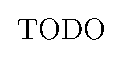
\includegraphics[width=\textwidth]{TODO}
        \caption{An original graph with highlighted biconnected componnents and cut vertices}
        \label{fig:bidec:original_graph}
    \end{subfigure}
    \hfill
    \begin{subfigure}{0.4\textwidth}
        \centering
        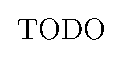
\includegraphics[width=\textwidth]{TODO}
        \caption{Block-cut tree of a graph}
        \label{fig:bidec:bctree}
    \end{subfigure}
    \hfill
    \begin{subfigure}{0.4\textwidth}
        \centering
        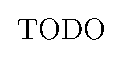
\includegraphics[width=\textwidth]{TODO}
        \caption{Outer \(k\)-planar drawing of each componnent}
        \label{fig:bidec:componnents_drawings}
    \end{subfigure}
    \hfill
    \begin{subfigure}{0.4\textwidth}
        \centering
        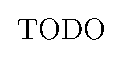
\includegraphics[width=\textwidth]{TODO}
        \caption{Outer \(k\)-planar drawing of the original graph}
        \label{fig:bidec:graph_drawing}
    \end{subfigure}
    \caption{An example of bicomponnent decomposition}
\end{figure}

For complex problems, decomposing into smaller subproblems often leads to a significant increase in performance. In our context of recognising outer \(k\)-planar graphs, an effective strategy to do so is to partition the graph into subgraphs in such a manner that allows us to process them independently by the recognition algorithm. One of the plausible ways to accomplish this is to split the graph into biconnected components as shown in the figure~\ref{fig:bidec:original_graph}. This process is implemented using block-cut decomposition. It is worth noting that each graph edge belongs to a single biconnected component, referred to as a block. However, any two bicomponents may share a vertex, referred to as a cut vertex. Considering blocks and cut vertices as graph nodes, we can construct a so-called block-cut tree, wherein a block node is connected to a cut node if and only if the corresponding biconnected component contains a corresponding vertex, see figure~\ref{fig:bidec:bctree}.

\todo[inline]{How to show that this boosts performance more formally in the next sentence?}

Due to the nature of bi-connectedness, after getting outer \(k\)-planar drawings of biconnected components separately, we can combine them easily into an outer \(k\)-planar drawing of the whole graph, hence, the increase in performance. To be more specific, if some component does not admit an outer \(k\)-planar drawing, neither does the whole graph. Otherwise, if all components admit such a drawing, they can be merged by combining duplicates of each cut vertex see figures~\ref{fig:bidec:componnents_drawings} and~\ref{fig:bidec:graph_drawing}. This merging process does not introduce any additional edge crossings since both components are located on the outer face of each other. Moreover, as no new faces are created during this process (due to the acyclic structure of the block-cut tree), every vertex remains on the outer face of the graph during this process. Consequently, the resulting drawing of an original graph is outer \(k\)-planar, and it exists if and only if each biconnected component of the graph admits such a drawing.

In this work, we implemented this decomposition using the method \textsf{bi\-connec\-ted\_compo\-nents}\footnote{\url{https://www.boost.org/doc/libs/1_87_0/libs/graph/doc/biconnected_components.html}} from the Boost Graph Library~\cite{boost}. This function assigns an index of the bicomponent to each edge to which it belongs. Additionally, it provides a list of cut vertices. Afterwards, we copy each block as an independent graph and create mappings to translate new \emph{local} vertices back to their original identifiers. Finally, we construct a supergraph representing the structure of a block-cut tree wherein each node references a copied block alongside corresponding mapping or a cut vertex.

To construct a drawing of the whole graph, after performing the decomposition, we perform a depth-first search on the block-cut tree, recording the predecessor for each node upon discovery. Additionally, each time a block vertex is discovered, we use one of the methods described in other sections of this chapter to check whether the component admits an outer \(k\)-planar drawing and obtain it if so. Afterwards, we merge the new drawing with the already existing one by combining the common cut vertex as described before. If the considered block is the first encountered one, its drawing is directly copied into a sequence that will form the final drawing. Otherwise, the block necessarily has a predecessor. Due to the structure of a tree, it is a cut node corresponding to a vertex that is shared with some other block that has already been considered and thus added to a final drawing. As a result, we can find a corresponding cut vertex in both global and local drawings. Since each drawing is represented as a cyclic sequence of vertices, we can rotate the local drawing so that the corresponding cut vertex appears as the first item in a sequence. Finally, we insert the local drawing starting from the second element into the global one immediately after the corresponding cut vertex.

\section{ILP Formulation (unchanged)}\label{sec:ILP-def}

The result of the integral linear program should be an arrangement of vertices on a line.
Given the arrangement of the vertices, we can definitively identify whether two edges cross each other.
Indeed, consider two edges, $uv$ and $st$.
Without loss of generality, we can assume that $u$ is located before $v$ in the arrangement, $s$ before $t$, and $u$ before $s$.
Under these assumptions, the edges $uv$ and $st$ cross if and only if $s$ is located before $v$ and $t$ after $v$.

\todo[inline]{Image depicting 8 intersecting pairs out of 24 possibble}

The arrangement is represented using the so-called ``ordering variables''.
For every pair of vertices $u$ and $v$, we create a binary variable $a_{u, v}$ that defines the order in which they appear in the arrangement.
Equality $a_{u, v} = 1$ indicates that $u$ is located before $v$ and vice versa, and $a_{u, v} = 0$ indicates that $v$ is located before $u$ or $u$ and $v$ is the same vertex.

For these variables, it is crucial to ensure transitivity.
That is, if $a_{u, v} = 1$ and $a_{v, w} = 1$ which means $u$ is located before $v$ and $v$ is located before $w$, then $u$ must be located before $w$, so the following should hold $a_{u, w} = 1$.
This can be ensured by the following constraint: $a_{u, w} \geqslant a_{u, v} + a_{v, w} - 1$.
This constraint will restrict the value of $a_{u, w}$ if and only if both $a_{u, v}$ and $a_{v, w}$ equal $1$.
Otherwise, the constraint will have no impact on the system at all.

Having the arrangement of the vertices, we can now deduce for each pair of edges $uv$ and $st$ whether they intersect or not.
Naturally, there are 24 different arrangements of the vertices, as demonstrated in figure~\ref{fig:edge_crossings}.
Among them, there are only eight in which the edges intersect.
Thus, the edge $uv$ crosses the edge $st$ if and only if one of the following holds:
\begin{itemize}[noitemsep]
    \item $a_{u,s} = 1$, $a_{s,v} = 1$, and $a_{v,t} = 1$
    \item $a_{u,t} = 1$, $a_{t,v} = 1$, and $a_{v,s} = 1$
    \item $a_{v,s} = 1$, $a_{s,u} = 1$, and $a_{u,t} = 1$
    \item $a_{v,t} = 1$, $a_{t,u} = 1$, and $a_{u,s} = 1$
    \item $a_{s,u} = 1$, $a_{u,t} = 1$, and $a_{t,v} = 1$
    \item $a_{t,u} = 1$, $a_{u,s} = 1$, and $a_{s,v} = 1$
    \item $a_{s,v} = 1$, $a_{v,t} = 1$, and $a_{t,u} = 1$
    \item $a_{t,v} = 1$, $a_{v,s} = 1$, and $a_{s,u} = 1$
\end{itemize}

To describe this in the linear program, we create a binary variable $c_{uv, st}$ for every pair of edges $uv$ and $st$.
Equality $c_{uv, st} = 0$ indicates that the edge $uv$ does not cross $st$.
To ensure the correctness of these values, we impose eight constraints on each variable, one for each case from above.
For example, considering the case $a_{u,s} = 1$, $a_{s,v} = 1$, and $a_{v,t} = 1$, we impose the following restriction: $c_{uv, st} \geqslant a_{u,s} + a_{s,v} + a_{v,t} - 2$, which ensures that $c_{uv, st}$ equals $1$ whenever the vertices are ordered as $usvt$.
Making this for each case restricts $c_{uv, st}$ to the value $1$ if the vertices are arranged in one of the eight ``intersecting'' configurations, ensuring that $c_{uv, st} = 0$ is possible only if $uv$ does not cross $st$.

The algorithm's objective is to minimize the maximal number of crossings per edge.
This value can be written as follows: $\max_{uv \in E(G)} \sum_{st \in E(G)} c_{uv, st}$.
Unfortunately, it cannot represent an objective function for a linear program as the $\max$ operation is not linear.
To solve this, we introduce a new integer variable $k$.
To ensure that it is equal to the objective value, we impose the following constraint on $k$: $k \geqslant \sum_{st \in E(G)} c_{uv, st}$ for each edge $uv \in E(G)$.

So, the integer linear program can be described as follows:
\begin{align*}
    \textbf{minimize}\quad&k\\
    \textbf{subject to}\quad&&k &\geqslant \sum_{st \in E(G)} c_{uv, st},&&\forall uv \in E(G)\\
    &&c_{uv, st} &\geqslant a_{u,s} + a_{s,v} + a_{v,t} - 2,&&\forall uv, st \in E(G)\\
    &&c_{uv, st} &\geqslant a_{u,t} + a_{t,v} + a_{v,s} - 2,&&\forall uv, st \in E(G)\\
    &&c_{uv, st} &\geqslant a_{v,s} + a_{s,u} + a_{u,t} - 2,&&\forall uv, st \in E(G)\\
    &&c_{uv, st} &\geqslant a_{v,t} + a_{t,u} + a_{u,s} - 2,&&\forall uv, st \in E(G)\\
    &&c_{uv, st} &\geqslant a_{s,u} + a_{u,t} + a_{t,v} - 2,&&\forall uv, st \in E(G)\\
    &&c_{uv, st} &\geqslant a_{t,u} + a_{u,s} + a_{s,v} - 2,&&\forall uv, st \in E(G)\\
    &&c_{uv, st} &\geqslant a_{s,v} + a_{v,t} + a_{t,u} - 2,&&\forall uv, st \in E(G)\\
    &&c_{uv, st} &\geqslant a_{t,v} + a_{v,s} + a_{s,u} - 2,&&\forall uv, st \in E(G)\\
    &&a_{u, w} &\geqslant a_{u, v} + a_{v, w} - 1,&&\forall u, v, w \in V(G)\\
    &&c_{uv, st} &\in \{0, 1\},&&\forall uv, st \in E(G)\\
    &&a_{u, v} &\in \{0, 1\},&&\forall u, v \in V(G)\\
\end{align*}


\section{SAT Formulation (unchanged)}\label{sec:SAT-def}

Another approach to solving this problem is to check for a specific $k$ whether the given graph is outer-$k$-planar.
This check can be encoded as a boolean satisfiability problem.
This problem asks whether it is possible to assign logic values $\textsc{True}$ or $\textsc{False}$ so that all disjunctive clauses are satisfied.
A disjunctive clause is a single literal or a disjunction of several.
Literal is either a variable or a negation of a variable, with the former being the positive and the latter the negative literal.


Similarly to the ILP algorithm described in~\ref{sec:ILP-def}, this algorithm uses the same ``ordering variables'' $a_{u, v}$ for each pair of vertices $u$ and $v$ that represent the arrangement of the vertices.
If the boolean variable $a_{u, v}$ is $\textsc{True}$, the vertex $u$ is located before the vertex $v$ and vice versa otherwise.

Similarly, these variables must account for transitivity, which means that for every triple of vertices $u$, $v$, and $w$ $a_{u, v} \equiv \textsc{True}$ and $a_{v, w} \equiv \textsc{True}$ implies $a_{u, w} \equiv \textsc{True}$.
This can be written as follows: $a_{u, v} \land a_{v, w} \rightarrow a_{u, w}$.
Expanding the implication, this transforms into $\overline{a_{u, v} \land a_{v, w}} \lor a_{u, w}$.
After applying De Morgan's law, we receive $\overline{a_{u, v}} \lor \overline{a_{v, w}} \lor a_{u, w}$, which represents a clause in the SAT problem.

The next step is to represent the crossing variables $c_{uv, st}$ in terms of the ordering ones for each pair of edges $uv$ and $st$.
Similarly to the ILP algorithm, we can restrict $c_{uv, st}$ to $\textsc{True}$ if $uv$ and $st$ cross by adding new clauses to the problem.
The clauses are constructed by making the implications for each of the eight intersecting cases shown in figure~\ref{fig:edge_crossings}, expanding them, and applying De Morgan's law.
For example, for the case $a_{u,s} = 1$, $a_{s,v} = 1$, and $a_{v,t} = 1$, we start with the logical equation as follows: $a_{u,s} \land a_{s,v} \land a_{v,t} \rightarrow c_{uv, st}$.
Afterwards, we expand the implication: $\overline{a_{u,s} \land a_{s,v} \land a_{v,t}} \lor c_{uv, st}$.
Finally, we apply De Morgan's law: $\overline{a_{u,s}} \lor \overline{a_{s,v}} \lor \overline{a_{v,t}} \lor c_{uv, st}$ receiving one of the eight clauses for $c_{uv, st}$.

% Help
The last step in the construction of the problem is to count the number of crossings for each edge.
The goal of this solver is to check whether the number of crossings can be smaller or equal to some constant $k$ for each edge.
To ensure this, we can build a set of clauses that prevent the problem from being satisfiable if the value $k$ is too small.
To do so, for every edge $e_0$, we consider all combinations of $e_1, e_2, \dots, e_{k+1}$ for each of which we construct the following clause: $\overline{c_{e_0, e_1}} \lor \overline{c_{e_0, e_2}} \lor \cdots\lor \overline{c_{e_0, e_{k+1}}}$.
Doing so, we ensure that for each edge $e_0$, no $k + 1$ different edges intersect $e_0$, which effectively means that each edge has at most $k$ crossings if all clauses are satisfied.

\todo[inline]{implementation details (iterate over all permutations, finding minimal k)}
\todo[inline]{possible optimizations (2k + 2, equivalence instead of implication for c\_\{...\}, eliminating c\_\{...\} at all)}


\section{Dynamic algorithm}

The last algorithm we considered was introduced by \citeauthor{okp}~\cite{okp}. Its core idea is to build the drawing incrementally. Each step of this process can be parameterised by three parameters. The first is a pair of vertices \(u\) and \(v\) that split a potential drawing into two parts, denoted as a link. The next is a set \(R_{uv}\) of vertices lying to the right of the split. And lastly the set \(E_{uv} = \{e_1, e_2, \dots, e_l\}\) of \(l\) edges crossing the \(uv\) link from the right to the left side. Let \(G_{uv, R_{uv}}\) be a graph consisting of vertices \(\{u, v\} \cup R_{uv}\) alongside all connecting edges from an original graph \(G\) with inserted vertices \(t_1, t_2, \dots, t_l\) connected to corresponding vertices by edges \(e_1, e_2, \dots, e_l\). We call a configuration on each step \emph{drawable} if exists an outer \(k\)-planar drawing of a corresponding graph \(G_{uv, R_{uv}}\) which cyclic order contains \((u, t_{\tau(1)}, t_{\tau(2)}, \dots, t_{\tau(l)}, v)\) as a consecutive subsequence for some permutation \(\tau\). On each step, the algorithm finds all possible permutations for which the configuration is \emph{drawable} and stores them in the lookup table.

To significantly reduce the search space, the authors used the result of \citeauthor{triangulations}. In their work~\cite{triangulations}, authors showed that the right side of any \emph{drawable} configuration can be split into two smaller parts by selecting a vertex \(w\) from the right side in such a way that both links \(uw\) and \(vw\) are crossed by at most \(k\) edges. This allows us to limit the search only to \emph{narrow} configurations with \(l \leqslant k\) as by reversing the argument, we get that outer \(k\)-planar drawing for \(G_{uv, R_{uv}}\) is possible if and only if we can combine it from two \emph{narrow drawable} configurations for active links \(uw\) and \(vw\) for some vertex \(w\) from the right side.

In the implementation of the algorithm, we first construct an index of all possible \emph{narrow} configurations. Since, on each step, we try to draw a configuration using two smaller \emph{drawable} ones, we grouped them by the size of the right part, guaranteeing that all smaller \emph{drawable} configurations are already discovered at any point. Since the amount of crossing edges is bounded by \(k\), the number of entries in this index can be bounded by the following amount:~\(2^{O(k)}m^{k+O(1)}\)~\cite[Lemma 15]{okp}.

To populate this index, we start by iterating over possible values for \(l\)\footnote{By iterating over this first, we ensure that it is easy to extend the index for \(k+1\) edges if the check for outer \(k\)-planarity is unsuccessful.}. For each choice of \(l\) and each link \(uv\), we consider an augmented graph \(H\) obtained by removing \(u\) and \(v\) from the original graph \(G\) alongside all connected edges. Then, we select exactly \(l\) edges from \(H\) to cross the link \(uv\). These edges further subdivide some connected components of \(H\) into connected subcomponents. Crucially, as these subcomponents do not contain edges that cross the link, each one of them must be located entirely on one side. Thus, finding all valid right sides for a given link means finding all valid black-white colourings of subcomponents, where white indicates belonging to the right and black to the left side. Consequently, each selected edge has to connect subcomponents of different colours, or in other words, the metagraph of each connected component of \(H\) with subcomponents as vertices connected by selected edges has to be bipartite. After ensuring this holds, we construct all possible right sides for the selected link. As each bipartite graph can be coloured in exactly two ways, there are exactly \(2^d\) possible right sides, where \(d\) is the number of connected components in graph \(H\). As a result, there might be a massive number of entries in the index and, consequently, the lookup table itself. To minimise the memory consumption and make it feasible, we represent the right sides as binary masks stored as 64-bit integers. This decision limits the current implementation to graphs with at most 64 vertices. However, considering the complexity of the algorithm, we believe the graphs of this size would require an unreasonable amount of resources anyway\footnote{Potentially it is possible to develop a specified bitmask object which could handle any number of vertices by using multiple integers stored in an array.}.

In the lookup table itself, for each configuration, we record all discovered sets of arrangements of \(E_{uv}\) that can appear in an outer \(k\)-planar drawing of \(G_{uv, R_{uv}}\) grouped by the link \(uv\) and the right side \(R_{uv}\). Each arrangement \(A_{uv}\)\footnote{I think I should use another letter} consist of a permutation \(\tau\) of edges in \(E_{uv}\) and a map \(f_{uv}:E_{uv}\rightarrow \mathbb{N}_+\) that matches each edge from \(E_{uv}\) with its number of intersections in the drawing of \(G_{uv, R_{uv}}\).

Next, iterating over the index, we fill the corresponding cells of the lookup table. For that, we have to find all arrangements for which a specific configuration is \emph{drawable}. We start by selecting a split vertex \(w\) that belongs to the right side \(R_{uv}\). For each \(w\), we iterate over all configurations for a link \(uw\) with a right side \(R_{uw}\) being a subset of \(R_{uv}\). At the same time, we also consider a complementary configuration with a link \(vw\) and right side \(R_{vw} = R_{uv} \setminus (R_{uw} \cup \{w\})\). For each such pair of configurations, we iterate over all pairs of \emph{drawable} arrangements \(A_{uw}\) and \(A_{vw}\) saved in the lookup table and search for all possible ways to combine them into an outer \(k\)-planar drawing of \(G_{uv, R_{uv}}\).

There is only one way to glue drawings of two configurations together. However, to form a valid drawing of \(G_{uv, R_{uv}}\), we also have to decide on the order of edges crossing the link \(uv\) represented by a permutation \(\tau_{uv}\). To ensure the correctness of the solution, we go through all possible ones. For each permutation, we check whether the resulting drawing is valid~--~each edge is crossed at most \(k\) times. To do so, we focus on an inner triangle consisting of three vertices \(u\), \(v\) and \(w\), and all the edges crossing at least one of the links \(uv\), \(uw\) and \(vw\). Additionally, we include edge \((u, v)\) if such exists. Crucially, to calculate all the intersections apart from the edges, we also need the order in which they enter the triangle. As sides of the triangle are exactly the links, this order is represented in corresponding permutations: \(\tau_{uw}\) from \(A_{uw}\), \(\tau_{vw}\) from \(A_{vw}\) and \(\tau_{uv}\) which are looked through one by one. To represent this in the triangle, we insert \(l_{uv}\) helper vertices between \(u\) and \(v\), given that \(l_{uv}\) is a size of \(E_{uv}\), and treat them as endpoints of edges that cross the link \(uv\). Similarly, we insert vertices corresponding to edges crossing \(uw\) and \(vw\). Importantly, each inserted vertex is an endpoint only for one edge and is ordered according to the corresponding permutations. By considering these vertices as edges' endpoints, we limit the view to the intersections created by the combination of two parts, ignoring those in \(R_{uw}\) and \(R_{vw}\). So, to get the crossing number for each edge, apart from the ones we count in the triangle, we also have to add those accounted by \(f_{uw}\) and \(f_{vw}\). If the crossing number of any edge exceeds \(k\), we discard the permutation \(\tau_{uv}\) and proceed to the next one. Otherwise, we add a new arrangement to the lookup table.

If at any moment, the algorithm finds a \emph{drawable} configuration for vertices \(u\) and \(v\) with \(R_{uv} = V(G)\setminus\{u, v\}\), it halts indicating that \(G\) is outer \(k\)-planar, as in such a case \(G_{uv, R_{uv}}\) is an original graph \(G\) and admits an outer \(k\)-planar drawing. If, on the other hand, the lookup table is filled, and no such configuration is found, the algorithm halts, indicating that the graph is not outer \(k\)-planar. Similar to the SAT-based algorithm from the section~\ref{sec:SAT-def}, this method only tests whether the graph admits outer \(k\)-planar drawing or not for a fixed \(k\), so to find the minimal possible crossing number we have to check the values incrementally.
